% Mémoire v1.1 : mise à jour des résultats (2026-08-24)
% Compilé avec tectonic ; tableaux générés par scripts/make_latex_tables.py, figures par mlrp figures / mlrp shap.
\documentclass[11pt]{article}
\usepackage[T1]{fontenc}
\usepackage{amsmath,graphicx,mathtools,amssymb}
\usepackage[table]{xcolor}
\definecolor{Gray}{gray}{0.9}
\definecolor{Green}{rgb}{0,0.5,0}
\usepackage{booktabs,colortbl,geometry}
\usepackage[french]{babel}
\geometry{hmargin=2cm,vmargin=2.5cm}
\usepackage{siunitx}
\usepackage{array,makecell}
\usepackage[hidelinks]{hyperref}
\usepackage{caption}
\captionsetup{font=small}

\title{Évaluation empirique d'actifs canadiens par l'apprentissage automatique\\
\large Version 1.1 : résultats mis à jour\\
\normalsize Mise à jour du mémoire de maîtrise (UQAM, décembre 2024)}
\author{Guillaume Vaudescal}
\date{24 août 2026}

\begin{document}
\maketitle

\section*{Ce qui change entre le mémoire de 2024 et cette version 1.1}

Cette mise à jour ne change ni la question de recherche, ni les données macroéconomiques, ni les huit modèles,
ni la procédure d'entraînement. Elle corrige quatre points d'implémentation et de présentation, puis régénère
tous les tableaux et toutes les figures avec le pipeline vérifié de 2026
(\url{https://github.com/Guilou001/memoire-uqam-2024}, paquet \texttt{mlrp}) :

\begin{enumerate}
  \item \textbf{Le portefeuille long short soustrait désormais réellement le côté short.} Le code de 2024
  additionnait la contribution du panier short au lieu de la soustraire : les portefeuilles publiés étaient
  longs des deux côtés (exposition brute de 200~\%). Les résultats ci-dessous appliquent la stratégie telle que
  décrite au chapitre~3 du mémoire (long les mieux classés, short les moins bien classés).
  \item \textbf{Le TCAC est calculé en années civiles.} La version 2024 de la bibliothèque de métriques divisait
  les jours civils par 252, ce qui sous-estimait le rendement annualisé.
  \item \textbf{L'univers canadien compte 50 titres cotés sur toute la période.} La liste de 2024 contenait un
  doublon (ENB.TO) et un FNB (XIU.TO) ; CNQ.TO (Canadian Natural Resources) et GIB-A.TO (CGI) les remplacent.
  \item \textbf{Un rééquilibrage dont le 1\textsuperscript{er} du mois n'est pas un jour de bourse est appliqué
  au jour de bourse suivant} (le code de 2024 le sautait).
\end{enumerate}

Deux limites connues restent volontairement en l'état pour préserver la comparabilité avec le mémoire, et sont
mesurées dans le dépôt : les hyperparamètres sont choisis sur la période de test, et les variables
macroéconomiques sont alignées un mois en avance sur le rendement prédit. Leur correction est le chantier de la
version~2. Enfin, plusieurs modèles produisent des prédictions identiques pour tous les titres à la plupart des
dates (Extra Trees en tête, dont l'élagage retenu réduit chaque arbre à une feuille) ; leurs lignes mesurent
alors un portefeuille quasi fixe et non un classement, ce que le lecteur doit garder en tête.

% ------------------------------------------------------------------ résultats
\clearpage
\section*{Résultats mis à jour}

% PROSE_RESULTATS : rédigée par scripts/make_v11_prose.py une fois le run complet terminé
% Généré par scripts/make_v11_prose.py, ne pas éditer à la main.

\subsection*{Période 2008-01 à 2024-01}

Aux États-Unis, sur les huit portefeuilles long short top~10, 6 affichent un TCAC positif. Le meilleur est le Hist Gradient Boosting, avec 7,4~\% par an (Sharpe 0,80, perte maximale 18,1~\%). Sur la même période, le S\&P 500 rend 7,6~\% (Sharpe 0,46) et le portefeuille équipondéré des titres de l'univers 10,8~\% (Sharpe 0,64) ; 3 portefeuille(s) long short sur huit font mieux que l'équipondéré en Sharpe.

Au Canada, sur les huit portefeuilles long short top~10, 2 affichent un TCAC positif. Le meilleur est le XGBoost, avec 5,6~\% par an (Sharpe 0,39, perte maximale 35,4~\%). Sur la même période, le composite TSX rend 2,6~\% (Sharpe 0,24) et le portefeuille équipondéré des titres de l'univers 11,5~\% (Sharpe 0,78) ; 0 portefeuille(s) long short sur huit font mieux que l'équipondéré en Sharpe.

Les $R^2$ hors échantillon moyens des régressions restent négatifs ou nuls (de $-$0,55 à 0,00 côté américain) : les prédictions expliquent moins bien les rendements qu'une moyenne simple, et la valeur des portefeuilles vient du classement, non du niveau prédit. Les modèles dont les prédictions sont identiques pour tous les titres à la plupart des dates (voir \texttt{results/v2/tables/prediction\_ties.csv}) doivent se lire comme des portefeuilles quasi fixes.

\subsection*{Période 2008-01 à 2012-01}

Aux États-Unis, sur les huit portefeuilles long short top~10, 7 affichent un TCAC positif. Le meilleur est le XGBoost, avec 10,8~\% par an (Sharpe 0,72, perte maximale 25,0~\%). Sur la même période, le S\&P 500 rend $-$3,8~\% (Sharpe 0,01) et le portefeuille équipondéré des titres de l'univers 4,4~\% (Sharpe 0,30) ; 7 portefeuille(s) long short sur huit font mieux que l'équipondéré en Sharpe.

Au Canada, sur les huit portefeuilles long short top~10, 2 affichent un TCAC positif. Le meilleur est le XGBoost de classification, avec 7,7~\% par an (Sharpe 0,53, perte maximale 13,4~\%). Sur la même période, le composite TSX rend $-$3,6~\% (Sharpe $-$0,01) et le portefeuille équipondéré des titres de l'univers 5,2~\% (Sharpe 0,35) ; 1 portefeuille(s) long short sur huit font mieux que l'équipondéré en Sharpe.

Les $R^2$ hors échantillon moyens des régressions restent négatifs ou nuls (de $-$0,46 à $-$0,00 côté américain) : les prédictions expliquent moins bien les rendements qu'une moyenne simple, et la valeur des portefeuilles vient du classement, non du niveau prédit. Les modèles dont les prédictions sont identiques pour tous les titres à la plupart des dates (voir \texttt{results/v2/tables/prediction\_ties.csv}) doivent se lire comme des portefeuilles quasi fixes.

\subsection*{Période 2012-01 à 2020-01}

Aux États-Unis, sur les huit portefeuilles long short top~10, 5 affichent un TCAC positif. Le meilleur est le XGBoost, avec 7,5~\% par an (Sharpe 0,90, perte maximale 15,1~\%). Sur la même période, le S\&P 500 rend 12,5~\% (Sharpe 0,99) et le portefeuille équipondéré des titres de l'univers 14,5~\% (Sharpe 1,17) ; 0 portefeuille(s) long short sur huit font mieux que l'équipondéré en Sharpe.

Au Canada, sur les huit portefeuilles long short top~10, 3 affichent un TCAC positif. Le meilleur est la régression logistique, avec 2,5~\% par an (Sharpe 0,24, perte maximale 24,7~\%). Sur la même période, le composite TSX rend 4,6~\% (Sharpe 0,47) et le portefeuille équipondéré des titres de l'univers 14,4~\% (Sharpe 1,42) ; 0 portefeuille(s) long short sur huit font mieux que l'équipondéré en Sharpe.

Les $R^2$ hors échantillon moyens des régressions restent négatifs ou nuls (de $-$0,16 à $-$0,04 côté américain) : les prédictions expliquent moins bien les rendements qu'une moyenne simple, et la valeur des portefeuilles vient du classement, non du niveau prédit. Les modèles dont les prédictions sont identiques pour tous les titres à la plupart des dates (voir \texttt{results/v2/tables/prediction\_ties.csv}) doivent se lire comme des portefeuilles quasi fixes.

\subsection*{Période 2020-01 à 2024-01}

Aux États-Unis, sur les huit portefeuilles long short top~10, 7 affichent un TCAC positif. Le meilleur est le XGBoost de classification, avec 6,5~\% par an (Sharpe 0,66, perte maximale 17,1~\%). Sur la même période, le S\&P 500 rend 10,3~\% (Sharpe 0,54) et le portefeuille équipondéré des titres de l'univers 9,4~\% (Sharpe 0,54) ; 4 portefeuille(s) long short sur huit font mieux que l'équipondéré en Sharpe.

Au Canada, sur les huit portefeuilles long short top~10, 3 affichent un TCAC positif. Le meilleur est le XGBoost, avec 6,9~\% par an (Sharpe 0,41, perte maximale 45,1~\%). Sur la même période, le composite TSX rend 5,3~\% (Sharpe 0,36) et le portefeuille équipondéré des titres de l'univers 11,6~\% (Sharpe 0,66) ; 0 portefeuille(s) long short sur huit font mieux que l'équipondéré en Sharpe.

Les $R^2$ hors échantillon moyens des régressions restent négatifs ou nuls (de $-$1,21 à $-$0,14 côté américain) : les prédictions expliquent moins bien les rendements qu'une moyenne simple, et la valeur des portefeuilles vient du classement, non du niveau prédit. Les modèles dont les prédictions sont identiques pour tous les titres à la plupart des dates (voir \texttt{results/v2/tables/prediction\_ties.csv}) doivent se lire comme des portefeuilles quasi fixes.


\clearpage
\begin{table}[h]
\centering
\small
\caption{Résumé statistique des portefeuilles long short, 2008-01/2024-01 (régression)}
\vspace{.2cm}
\resizebox{\textwidth}{!}{%
\begin{tabular}{l *{6}{S[table-format=3.2]} | *{6}{S[table-format=3.2]}}
\toprule
\midrule
& \multicolumn{6}{c}{Canada} & \multicolumn{6}{c}{États-Unis} \\
\cmidrule(lr){2-7} \cmidrule(lr){8-13}
& \textit{\(R^2_{\text{HÉ}}\)} & \textit{\(r^A\)} & \textit{SR} & \textit{ST} & \textit{P\,$^{\text{max}}$} & \textit{$\Omega$} & \textit{\(R^2_{\text{HÉ}}\)} & \textit{\(r^A\)} & \textit{SR} & \textit{ST} & \textit{P\,$^{\text{max}}$} & \textit{$\Omega$} \\
\midrule
\rowcolor{Gray}
\textbf{Long short 10} &  &  &  &  &  &  &  &  &  &  &  & \\
\addlinespace[0.1cm]
Ridge & -1,28 & -6,62 & -0,29 & -0,40 & \bfseries\color{Green}75,78 & 0,95 & -0,40 & -0,92 & -0,00 & -0,01 & 44,58 & 1,00 \\ \addlinespace[0.1cm]
XGBoost & \bfseries\color{Green}0,03 & \bfseries\color{Green}5,63 & \bfseries\color{Green}0,39 & \bfseries\color{Green}0,57 & 35,37 & \bfseries\color{Green}1,07 & -0,20 & -0,58 & 0,02 & 0,03 & \bfseries\color{Green}57,88 & 1,00 \\ \addlinespace[0.1cm]
Ada Boost & -0,10 & 1,32 & 0,16 & 0,23 & 46,16 & 1,03 & -0,55 & 0,45 & 0,10 & 0,14 & 33,56 & 1,02 \\ \addlinespace[0.1cm]
Extra Trees & 0,01 & -3,54 & -0,13 & -0,19 & 56,76 & 0,98 & \bfseries\color{Green}0,00 & \bfseries\color{Green}6,95 & \bfseries\color{Green}0,76 & \bfseries\color{Green}1,10 & 19,64 & \bfseries\color{Green}1,14 \\ \addlinespace[0.1cm]
\rowcolor{Gray}
\textbf{Long short 20} &  &  &  &  &  &  &  &  &  &  &  & \\
\addlinespace[0.1cm]
Ridge & -1,28 & -3,13 & -0,21 & -0,29 & \bfseries\color{Green}54,98 & 0,96 & -0,40 & -0,52 & -0,01 & -0,01 & 39,30 & 1,00 \\ \addlinespace[0.1cm]
XGBoost & \bfseries\color{Green}0,03 & \bfseries\color{Green}3,18 & \bfseries\color{Green}0,33 & \bfseries\color{Green}0,46 & 28,18 & \bfseries\color{Green}1,06 & -0,20 & 2,03 & 0,25 & 0,35 & \bfseries\color{Green}44,46 & 1,05 \\ \addlinespace[0.1cm]
Ada Boost & -0,10 & -1,08 & -0,04 & -0,05 & 38,59 & 0,99 & -0,55 & 1,49 & 0,22 & 0,31 & 22,76 & 1,04 \\ \addlinespace[0.1cm]
Extra Trees & 0,01 & -1,74 & -0,13 & -0,18 & 36,30 & 0,98 & \bfseries\color{Green}0,00 & \bfseries\color{Green}4,01 & \bfseries\color{Green}0,58 & \bfseries\color{Green}0,83 & 16,62 & \bfseries\color{Green}1,10 \\ \addlinespace[0.1cm]
\rowcolor{Gray}
\textbf{Long short $\gtrless$ 0} &  &  &  &  &  &  &  &  &  &  &  & \\
\addlinespace[0.1cm]
Ridge & -1,28 & 9,14 & 0,59 & 0,86 & 30,57 & 1,13 & -0,40 & \bfseries\color{Green}10,80 & \bfseries\color{Green}0,65 & \bfseries\color{Green}0,93 & 37,72 & \bfseries\color{Green}1,14 \\ \addlinespace[0.1cm]
XGBoost & \bfseries\color{Green}0,03 & -4,34 & -0,04 & -0,05 & \bfseries\color{Green}80,20 & 0,99 & -0,20 & -0,05 & 0,09 & 0,12 & \bfseries\color{Green}55,42 & 1,02 \\ \addlinespace[0.1cm]
Ada Boost & -0,10 & -1,06 & 0,06 & 0,09 & 66,54 & 1,01 & -0,55 & 4,28 & 0,32 & 0,44 & 36,57 & 1,07 \\ \addlinespace[0.1cm]
Extra Trees & 0,01 & \bfseries\color{Green}11,45 & \bfseries\color{Green}0,78 & \bfseries\color{Green}1,08 & 38,45 & \bfseries\color{Green}1,16 & \bfseries\color{Green}0,00 & 10,79 & 0,64 & 0,92 & 42,34 & 1,14 \\ \addlinespace[0.1cm]
\rowcolor{Gray}
\textbf{Critères de références} &  &  &  &  &  &  &  &  &  &  &  & \\
\addlinespace[0.1cm]
Même pondération &  & 11,86 & 0,80 &  &  &  &  & 11,08 & 0,66 &  &  &  \\ \addlinespace[0.1cm]
Indice (TSX / S\&P 500) &  & 2,63 & 0,24 &  &  &  &  & 11,45 & 0,59 &  &  &  \\ \addlinespace[0.1cm]
\bottomrule
\end{tabular}}
\end{table}

\begin{table}[h]
\centering
\small
\caption{Résumé statistique des portefeuilles long short, 2008-01/2024-01 (classification)}
\vspace{.2cm}
\resizebox{\textwidth}{!}{%
\begin{tabular}{l *{7}{S[table-format=3.2]} | *{7}{S[table-format=3.2]}}
\toprule
\midrule
& \multicolumn{7}{c}{Canada} & \multicolumn{7}{c}{États-Unis} \\
\cmidrule(lr){2-8} \cmidrule(lr){9-15}
& \textit{SP} & \textit{PT} & \textit{\(r^A\)} & \textit{SR} & \textit{ST} & \textit{P\,$^{\text{max}}$} & \textit{$\Omega$} & \textit{SP} & \textit{PT} & \textit{\(r^A\)} & \textit{SR} & \textit{ST} & \textit{P\,$^{\text{max}}$} & \textit{$\Omega$} \\
\midrule
\rowcolor{Gray}
\textbf{Long short 10} &  &  &  &  &  &  &  &  &  &  &  &  &  & \\
\addlinespace[0.1cm]
Régression logistique & 0,55 & 0,22 & -2,93 & -0,10 & -0,14 & 51,28 & 0,98 & 0,56 & 0,19 & 6,71 & 0,72 & 1,04 & 24,78 & 1,13 \\ \addlinespace[0.1cm]
XGBoost Classification & 0,59 & 0,12 & \bfseries\color{Green}-1,48 & \bfseries\color{Green}-0,01 & \bfseries\color{Green}-0,01 & 48,23 & \bfseries\color{Green}1,00 & 0,51 & 0,52 & 4,88 & 0,52 & 0,75 & 20,43 & 1,09 \\ \addlinespace[0.1cm]
Hist Gradient Boosting Classification & \bfseries\color{Green}0,62 & \bfseries\color{Green}0,05$^{*}$ & -1,58 & -0,01 & -0,02 & \bfseries\color{Green}47,95 & 1,00 & \bfseries\color{Green}0,58 & \bfseries\color{Green}0,10$^{*}$ & \bfseries\color{Green}7,42 & \bfseries\color{Green}0,80 & \bfseries\color{Green}1,17 & 18,11 & \bfseries\color{Green}1,14 \\ \addlinespace[0.1cm]
Extra Trees Classification & 0,56 & 0,34 & -3,54 & -0,13 & -0,19 & 56,76 & 0,98 & 0,52 & 0,72 & 5,61 & 0,63 & 0,90 & \bfseries\color{Green}17,40 & 1,11 \\ \addlinespace[0.1cm]
\rowcolor{Gray}
\textbf{Long short 20} &  &  &  &  &  &  &  &  &  &  &  &  &  & \\
\addlinespace[0.1cm]
Régression logistique & 0,55 & 0,22 & -1,75 & -0,13 & -0,18 & 40,25 & 0,98 & 0,56 & 0,19 & 3,81 & 0,55 & 0,79 & 16,62 & 1,10 \\ \addlinespace[0.1cm]
XGBoost Classification & 0,59 & 0,12 & -1,83 & -0,13 & -0,19 & 39,17 & 0,98 & 0,51 & 0,52 & 3,79 & 0,57 & 0,82 & \bfseries\color{Green}14,43 & 1,10 \\ \addlinespace[0.1cm]
Hist Gradient Boosting Classification & \bfseries\color{Green}0,62 & \bfseries\color{Green}0,05$^{*}$ & \bfseries\color{Green}-0,56 & \bfseries\color{Green}-0,01 & \bfseries\color{Green}-0,01 & 37,24 & \bfseries\color{Green}1,00 & \bfseries\color{Green}0,58 & \bfseries\color{Green}0,10$^{*}$ & \bfseries\color{Green}4,54 & \bfseries\color{Green}0,65 & \bfseries\color{Green}0,95 & 19,41 & \bfseries\color{Green}1,12 \\ \addlinespace[0.1cm]
Extra Trees Classification & 0,56 & 0,34 & -1,74 & -0,13 & -0,18 & \bfseries\color{Green}36,30 & 0,98 & 0,52 & 0,72 & 3,69 & 0,54 & 0,77 & 16,62 & 1,09 \\ \addlinespace[0.1cm]
\rowcolor{Gray}
\textbf{Long short $\gtrless$ 0} &  &  &  &  &  &  &  &  &  &  &  &  &  & \\
\addlinespace[0.1cm]
Régression logistique & 0,55 & 0,22 & 2,34 & 0,22 & 0,31 & 42,81 & 1,05 & 0,56 & 0,19 & \bfseries\color{Green}5,77 & 0,41 & 0,58 & 26,95 & 1,09 \\ \addlinespace[0.1cm]
XGBoost Classification & 0,59 & 0,12 & \bfseries\color{Green}14,12 & \bfseries\color{Green}0,85 & 1,19 & 45,82 & \bfseries\color{Green}1,19 & 0,51 & 0,52 & -1,77 & -0,13 & -0,17 & 49,89 & 0,98 \\ \addlinespace[0.1cm]
Hist Gradient Boosting Classification & \bfseries\color{Green}0,62 & \bfseries\color{Green}0,05$^{*}$ & -1,60 & 0,09 & 0,11 & 71,05 & 1,02 & \bfseries\color{Green}0,58 & \bfseries\color{Green}0,10$^{*}$ & 5,69 & \bfseries\color{Green}0,48 & \bfseries\color{Green}0,70 & \bfseries\color{Green}23,66 & \bfseries\color{Green}1,10 \\ \addlinespace[0.1cm]
Extra Trees Classification & 0,56 & 0,34 & 12,44 & 0,83 & \bfseries\color{Green}1,22 & \bfseries\color{Green}31,57 & 1,18 & 0,52 & 0,72 & -1,65 & 0,00 & 0,00 & 50,43 & 1,00 \\ \addlinespace[0.1cm]
\rowcolor{Gray}
\textbf{Critères de références} &  &  &  &  &  &  &  &  &  &  &  &  &  & \\
\addlinespace[0.1cm]
Même pondération &  &  & 11,45 & 0,78 &  &  &  &  &  & 10,79 & 0,64 &  &  &  \\ \addlinespace[0.1cm]
Indice (TSX / S\&P 500) &  &  & 2,63 & 0,24 &  &  &  &  &  & 7,65 & 0,46 &  &  &  \\ \addlinespace[0.1cm]
\bottomrule
\end{tabular}}
\end{table}

\clearpage
\begin{table}[h]
\centering
\small
\caption{Résumé statistique des portefeuilles long short, 2008-01/2012-01 (régression)}
\vspace{.2cm}
\resizebox{\textwidth}{!}{%
\begin{tabular}{l *{6}{S[table-format=3.2]} | *{6}{S[table-format=3.2]}}
\toprule
\midrule
& \multicolumn{6}{c}{Canada} & \multicolumn{6}{c}{États-Unis} \\
\cmidrule(lr){2-7} \cmidrule(lr){8-13}
& \textit{\(R^2_{\text{HÉ}}\)} & \textit{\(r^A\)} & \textit{SR} & \textit{ST} & \textit{P\,$^{\text{max}}$} & \textit{$\Omega$} & \textit{\(R^2_{\text{HÉ}}\)} & \textit{\(r^A\)} & \textit{SR} & \textit{ST} & \textit{P\,$^{\text{max}}$} & \textit{$\Omega$} \\
\midrule
\rowcolor{Gray}
\textbf{Long short 10} &  &  &  &  &  &  &  &  &  &  &  & \\
\addlinespace[0.1cm]
Ridge & -1,21 & -13,91 & -0,66 & -0,86 & \bfseries\color{Green}60,39 & 0,89 & -0,44 & -7,62 & -0,47 & -0,63 & \bfseries\color{Green}43,92 & 0,92 \\ \addlinespace[0.1cm]
XGBoost & -0,11 & -3,54 & -0,13 & -0,18 & 36,02 & 0,98 & -0,25 & \bfseries\color{Green}10,75 & \bfseries\color{Green}0,72 & \bfseries\color{Green}1,07 & 24,99 & \bfseries\color{Green}1,13 \\ \addlinespace[0.1cm]
Ada Boost & -0,05 & \bfseries\color{Green}2,28 & \bfseries\color{Green}0,21 & \bfseries\color{Green}0,30 & 33,94 & \bfseries\color{Green}1,04 & -0,46 & 6,16 & 0,52 & 0,77 & 14,42 & 1,09 \\ \addlinespace[0.1cm]
Extra Trees & \bfseries\color{Green}0,01 & -11,31 & -0,59 & -0,83 & 47,15 & 0,90 & \bfseries\color{Green}-0,00 & 7,08 & 0,69 & 1,04 & 15,19 & 1,12 \\ \addlinespace[0.1cm]
\rowcolor{Gray}
\textbf{Long short 20} &  &  &  &  &  &  &  &  &  &  &  & \\
\addlinespace[0.1cm]
Ridge & -1,21 & -8,16 & -0,57 & -0,75 & \bfseries\color{Green}47,46 & 0,90 & -0,44 & -2,79 & -0,22 & -0,30 & \bfseries\color{Green}26,14 & 0,96 \\ \addlinespace[0.1cm]
XGBoost & -0,11 & -1,93 & -0,12 & -0,17 & 21,67 & 0,98 & -0,25 & \bfseries\color{Green}8,20 & \bfseries\color{Green}0,80 & \bfseries\color{Green}1,16 & 14,14 & \bfseries\color{Green}1,14 \\ \addlinespace[0.1cm]
Ada Boost & -0,05 & \bfseries\color{Green}0,34 & \bfseries\color{Green}0,09 & \bfseries\color{Green}0,13 & 25,79 & \bfseries\color{Green}1,02 & -0,46 & 6,59 & 0,71 & 1,02 & 12,79 & 1,13 \\ \addlinespace[0.1cm]
Extra Trees & \bfseries\color{Green}0,01 & -6,65 & -0,60 & -0,85 & 30,83 & 0,90 & \bfseries\color{Green}-0,00 & 4,75 & 0,57 & 0,82 & 16,62 & 1,10 \\ \addlinespace[0.1cm]
\rowcolor{Gray}
\textbf{Long short $\gtrless$ 0} &  &  &  &  &  &  &  &  &  &  &  & \\
\addlinespace[0.1cm]
Ridge & -1,21 & \bfseries\color{Green}7,71 & \bfseries\color{Green}0,48 & \bfseries\color{Green}0,70 & 30,57 & \bfseries\color{Green}1,09 & -0,44 & -3,21 & -0,02 & -0,03 & 51,94 & 1,00 \\ \addlinespace[0.1cm]
XGBoost & -0,11 & -4,07 & -0,17 & -0,23 & 30,48 & 0,97 & -0,25 & -3,07 & -0,04 & -0,06 & 33,99 & 0,99 \\ \addlinespace[0.1cm]
Ada Boost & -0,05 & -0,40 & 0,14 & 0,20 & \bfseries\color{Green}43,43 & 1,03 & -0,46 & -0,48 & 0,13 & 0,18 & \bfseries\color{Green}59,37 & 1,03 \\ \addlinespace[0.1cm]
Extra Trees & \bfseries\color{Green}0,01 & 5,17 & 0,35 & 0,49 & 38,45 & 1,07 & \bfseries\color{Green}-0,00 & \bfseries\color{Green}4,40 & \bfseries\color{Green}0,30 & \bfseries\color{Green}0,42 & 42,34 & \bfseries\color{Green}1,06 \\ \addlinespace[0.1cm]
\rowcolor{Gray}
\textbf{Critères de références} &  &  &  &  &  &  &  &  &  &  &  & \\
\addlinespace[0.1cm]
Même pondération &  & 6,62 & 0,42 &  &  &  &  & 5,39 & 0,33 &  &  &  \\ \addlinespace[0.1cm]
Indice (TSX / S\&P 500) &  & -3,59 & -0,01 &  &  &  &  & -0,45 & 0,13 &  &  &  \\ \addlinespace[0.1cm]
\bottomrule
\end{tabular}}
\end{table}

\begin{table}[h]
\centering
\small
\caption{Résumé statistique des portefeuilles long short, 2008-01/2012-01 (classification)}
\vspace{.2cm}
\resizebox{\textwidth}{!}{%
\begin{tabular}{l *{7}{S[table-format=3.2]} | *{7}{S[table-format=3.2]}}
\toprule
\midrule
& \multicolumn{7}{c}{Canada} & \multicolumn{7}{c}{États-Unis} \\
\cmidrule(lr){2-8} \cmidrule(lr){9-15}
& \textit{SP} & \textit{PT} & \textit{\(r^A\)} & \textit{SR} & \textit{ST} & \textit{P\,$^{\text{max}}$} & \textit{$\Omega$} & \textit{SP} & \textit{PT} & \textit{\(r^A\)} & \textit{SR} & \textit{ST} & \textit{P\,$^{\text{max}}$} & \textit{$\Omega$} \\
\midrule
\rowcolor{Gray}
\textbf{Long short 10} &  &  &  &  &  &  &  &  &  &  &  &  &  & \\
\addlinespace[0.1cm]
Régression logistique & 0,57 & 0,27 & -11,77 & -0,60 & -0,85 & 42,55 & 0,90 & 0,54 & \bfseries\color{Green}0,31 & 7,99 & 0,77 & 1,15 & 15,80 & 1,14 \\ \addlinespace[0.1cm]
XGBoost Classification & 0,61 & 0,22 & \bfseries\color{Green}7,69 & \bfseries\color{Green}0,53 & \bfseries\color{Green}0,77 & \bfseries\color{Green}13,45 & \bfseries\color{Green}1,09 & 0,51 & 0,50 & 7,14 & 0,64 & 0,95 & 17,40 & 1,11 \\ \addlinespace[0.1cm]
Hist Gradient Boosting Classification & \bfseries\color{Green}0,62 & \bfseries\color{Green}0,13 & -5,15 & -0,19 & -0,26 & 31,19 & 0,97 & 0,52 & 0,46 & \bfseries\color{Green}9,56 & \bfseries\color{Green}0,84 & \bfseries\color{Green}1,31 & \bfseries\color{Green}9,19 & \bfseries\color{Green}1,16 \\ \addlinespace[0.1cm]
Extra Trees Classification & 0,55 & 0,35 & -11,31 & -0,59 & -0,83 & 47,15 & 0,90 & \bfseries\color{Green}0,55 & 0,35 & 7,22 & 0,71 & 1,05 & 15,19 & 1,13 \\ \addlinespace[0.1cm]
\rowcolor{Gray}
\textbf{Long short 20} &  &  &  &  &  &  &  &  &  &  &  &  &  & \\
\addlinespace[0.1cm]
Régression logistique & 0,57 & 0,27 & -6,00 & -0,52 & -0,73 & \bfseries\color{Green}25,41 & 0,91 & 0,54 & \bfseries\color{Green}0,31 & 3,83 & 0,47 & 0,68 & 16,62 & 1,08 \\ \addlinespace[0.1cm]
XGBoost Classification & 0,61 & 0,22 & -4,05 & -0,31 & -0,42 & 28,06 & 0,95 & 0,51 & 0,50 & 1,36 & 0,20 & 0,29 & 13,85 & 1,03 \\ \addlinespace[0.1cm]
Hist Gradient Boosting Classification & \bfseries\color{Green}0,62 & \bfseries\color{Green}0,13 & \bfseries\color{Green}-0,77 & \bfseries\color{Green}-0,01 & \bfseries\color{Green}-0,01 & 25,77 & \bfseries\color{Green}1,00 & 0,52 & 0,46 & 2,47 & 0,32 & 0,47 & \bfseries\color{Green}10,46 & 1,06 \\ \addlinespace[0.1cm]
Extra Trees Classification & 0,55 & 0,35 & -6,65 & -0,60 & -0,85 & 30,83 & 0,90 & \bfseries\color{Green}0,55 & 0,35 & \bfseries\color{Green}4,45 & \bfseries\color{Green}0,54 & \bfseries\color{Green}0,78 & 16,62 & \bfseries\color{Green}1,09 \\ \addlinespace[0.1cm]
\rowcolor{Gray}
\textbf{Long short $\gtrless$ 0} &  &  &  &  &  &  &  &  &  &  &  &  &  & \\
\addlinespace[0.1cm]
Régression logistique & 0,57 & 0,27 & 4,11 & 0,31 & 0,44 & 35,91 & 1,06 & 0,54 & \bfseries\color{Green}0,31 & \bfseries\color{Green}3,49 & \bfseries\color{Green}0,26 & \bfseries\color{Green}0,37 & \bfseries\color{Green}25,40 & \bfseries\color{Green}1,05 \\ \addlinespace[0.1cm]
XGBoost Classification & 0,61 & 0,22 & \bfseries\color{Green}9,15 & \bfseries\color{Green}0,54 & 0,75 & \bfseries\color{Green}20,00 & \bfseries\color{Green}1,11 & 0,51 & 0,50 & -6,60 & -0,37 & -0,51 & 47,26 & 0,93 \\ \addlinespace[0.1cm]
Hist Gradient Boosting Classification & \bfseries\color{Green}0,62 & \bfseries\color{Green}0,13 & -1,97 & 0,22 & 0,26 & 62,65 & 1,06 & 0,52 & 0,46 & -5,79 & -0,30 & -0,39 & 39,87 & 0,94 \\ \addlinespace[0.1cm]
Extra Trees Classification & 0,55 & 0,35 & 8,72 & 0,52 & \bfseries\color{Green}0,75 & 23,54 & 1,10 & \bfseries\color{Green}0,55 & 0,35 & -6,91 & -0,15 & -0,22 & 47,60 & 0,97 \\ \addlinespace[0.1cm]
\rowcolor{Gray}
\textbf{Critères de références} &  &  &  &  &  &  &  &  &  &  &  &  &  & \\
\addlinespace[0.1cm]
Même pondération &  &  & 5,17 & 0,35 &  &  &  &  &  & 4,40 & 0,30 &  &  &  \\ \addlinespace[0.1cm]
Indice (TSX / S\&P 500) &  &  & -3,59 & -0,01 &  &  &  &  &  & -3,81 & 0,01 &  &  &  \\ \addlinespace[0.1cm]
\bottomrule
\end{tabular}}
\end{table}

\clearpage
\begin{table}[h]
\centering
\small
\caption{Résumé statistique des portefeuilles long short, 2012-01/2020-01 (régression)}
\vspace{.2cm}
\resizebox{\textwidth}{!}{%
\begin{tabular}{l *{6}{S[table-format=3.2]} | *{6}{S[table-format=3.2]}}
\toprule
\midrule
& \multicolumn{6}{c}{Canada} & \multicolumn{6}{c}{États-Unis} \\
\cmidrule(lr){2-7} \cmidrule(lr){8-13}
& \textit{\(R^2_{\text{HÉ}}\)} & \textit{\(r^A\)} & \textit{SR} & \textit{ST} & \textit{P\,$^{\text{max}}$} & \textit{$\Omega$} & \textit{\(R^2_{\text{HÉ}}\)} & \textit{\(r^A\)} & \textit{SR} & \textit{ST} & \textit{P\,$^{\text{max}}$} & \textit{$\Omega$} \\
\midrule
\rowcolor{Gray}
\textbf{Long short 10} &  &  &  &  &  &  &  &  &  &  &  & \\
\addlinespace[0.1cm]
Ridge & -0,38 & -3,83 & -0,17 & -0,23 & 47,04 & 0,97 & -0,14 & -1,93 & -0,13 & -0,18 & 33,59 & 0,98 \\ \addlinespace[0.1cm]
XGBoost & -0,00 & -3,36 & -0,13 & -0,19 & 42,84 & 0,98 & \bfseries\color{Green}-0,04 & \bfseries\color{Green}7,51 & \bfseries\color{Green}0,90 & \bfseries\color{Green}1,31 & \bfseries\color{Green}15,11 & \bfseries\color{Green}1,16 \\ \addlinespace[0.1cm]
Ada Boost & -0,68 & -3,35 & -0,13 & -0,18 & 35,09 & 0,98 & -0,16 & -2,76 & -0,27 & -0,38 & 35,96 & 0,96 \\ \addlinespace[0.1cm]
Extra Trees & \bfseries\color{Green}0,01 & \bfseries\color{Green}0,40 & \bfseries\color{Green}0,10 & \bfseries\color{Green}0,15 & \bfseries\color{Green}27,92 & \bfseries\color{Green}1,02 & -0,05 & -0,84 & -0,05 & -0,06 & 21,14 & 0,99 \\ \addlinespace[0.1cm]
\rowcolor{Gray}
\textbf{Long short 20} &  &  &  &  &  &  &  &  &  &  &  & \\
\addlinespace[0.1cm]
Ridge & -0,38 & -0,98 & -0,05 & -0,07 & 24,22 & 0,99 & -0,14 & -1,52 & -0,18 & -0,24 & 27,36 & 0,97 \\ \addlinespace[0.1cm]
XGBoost & -0,00 & -2,22 & -0,18 & -0,25 & 33,95 & 0,97 & \bfseries\color{Green}-0,04 & \bfseries\color{Green}2,67 & \bfseries\color{Green}0,46 & \bfseries\color{Green}0,66 & 12,11 & \bfseries\color{Green}1,08 \\ \addlinespace[0.1cm]
Ada Boost & -0,68 & -5,79 & -0,54 & -0,75 & 43,68 & 0,91 & -0,16 & -0,79 & -0,10 & -0,14 & 27,52 & 0,98 \\ \addlinespace[0.1cm]
Extra Trees & \bfseries\color{Green}0,01 & \bfseries\color{Green}1,15 & \bfseries\color{Green}0,17 & \bfseries\color{Green}0,25 & \bfseries\color{Green}18,19 & \bfseries\color{Green}1,03 & -0,05 & 1,72 & 0,30 & 0,42 & \bfseries\color{Green}9,61 & 1,05 \\ \addlinespace[0.1cm]
\rowcolor{Gray}
\textbf{Long short $\gtrless$ 0} &  &  &  &  &  &  &  &  &  &  &  & \\
\addlinespace[0.1cm]
Ridge & -0,38 & 8,53 & 0,61 & 0,87 & 21,48 & 1,14 & -0,14 & 8,90 & 0,76 & 1,07 & 19,67 & 1,14 \\ \addlinespace[0.1cm]
XGBoost & -0,00 & -20,38 & -0,60 & -0,74 & 88,33 & 0,87 & \bfseries\color{Green}-0,04 & \bfseries\color{Green}12,25 & \bfseries\color{Green}1,01 & \bfseries\color{Green}1,42 & \bfseries\color{Green}16,75 & \bfseries\color{Green}1,20 \\ \addlinespace[0.1cm]
Ada Boost & -0,68 & -5,95 & -0,18 & -0,26 & 50,91 & 0,96 & -0,16 & 3,63 & 0,37 & 0,50 & 27,11 & 1,07 \\ \addlinespace[0.1cm]
Extra Trees & \bfseries\color{Green}0,01 & \bfseries\color{Green}14,37 & \bfseries\color{Green}1,42 & \bfseries\color{Green}2,08 & \bfseries\color{Green}13,86 & \bfseries\color{Green}1,27 & -0,05 & 10,45 & 0,87 & 1,22 & 24,56 & 1,17 \\ \addlinespace[0.1cm]
\rowcolor{Gray}
\textbf{Critères de références} &  &  &  &  &  &  &  &  &  &  &  & \\
\addlinespace[0.1cm]
Même pondération &  & 14,37 & 1,42 &  &  &  &  & 14,53 & 1,17 &  &  &  \\ \addlinespace[0.1cm]
Indice (TSX / S\&P 500) &  & 4,55 & 0,47 &  &  &  &  & 12,53 & 0,99 &  &  &  \\ \addlinespace[0.1cm]
\bottomrule
\end{tabular}}
\end{table}

\begin{table}[h]
\centering
\small
\caption{Résumé statistique des portefeuilles long short, 2012-01/2020-01 (classification)}
\vspace{.2cm}
\resizebox{\textwidth}{!}{%
\begin{tabular}{l *{7}{S[table-format=3.2]} | *{7}{S[table-format=3.2]}}
\toprule
\midrule
& \multicolumn{7}{c}{Canada} & \multicolumn{7}{c}{États-Unis} \\
\cmidrule(lr){2-8} \cmidrule(lr){9-15}
& \textit{SP} & \textit{PT} & \textit{\(r^A\)} & \textit{SR} & \textit{ST} & \textit{P\,$^{\text{max}}$} & \textit{$\Omega$} & \textit{SP} & \textit{PT} & \textit{\(r^A\)} & \textit{SR} & \textit{ST} & \textit{P\,$^{\text{max}}$} & \textit{$\Omega$} \\
\midrule
\rowcolor{Gray}
\textbf{Long short 10} &  &  &  &  &  &  &  &  &  &  &  &  &  & \\
\addlinespace[0.1cm]
Régression logistique & 0,54 & 0,40 & \bfseries\color{Green}2,54 & \bfseries\color{Green}0,24 & \bfseries\color{Green}0,36 & 24,71 & \bfseries\color{Green}1,04 & 0,57 & 0,29 & 4,89 & 0,59 & 0,83 & 17,19 & 1,11 \\ \addlinespace[0.1cm]
XGBoost Classification & 0,59 & 0,23 & -1,68 & -0,04 & -0,05 & 32,70 & 0,99 & 0,52 & 0,57 & 7,31 & 0,90 & \bfseries\color{Green}1,32 & 12,29 & 1,16 \\ \addlinespace[0.1cm]
Hist Gradient Boosting Classification & \bfseries\color{Green}0,69 & \bfseries\color{Green}0,00$^{***}$ & -3,66 & -0,17 & -0,24 & \bfseries\color{Green}40,79 & 0,97 & \bfseries\color{Green}0,66 & \bfseries\color{Green}0,04$^{**}$ & 6,69 & 0,79 & 1,14 & \bfseries\color{Green}23,04 & 1,14 \\ \addlinespace[0.1cm]
Extra Trees Classification & 0,58 & 0,38 & 0,17 & 0,09 & 0,13 & 29,24 & 1,01 & 0,61 & 0,50 & \bfseries\color{Green}7,51 & \bfseries\color{Green}0,90 & 1,31 & 15,11 & \bfseries\color{Green}1,16 \\ \addlinespace[0.1cm]
\rowcolor{Gray}
\textbf{Long short 20} &  &  &  &  &  &  &  &  &  &  &  &  &  & \\
\addlinespace[0.1cm]
Régression logistique & 0,54 & 0,40 & 0,44 & 0,09 & 0,14 & \bfseries\color{Green}24,59 & 1,02 & 0,57 & 0,29 & 2,04 & 0,35 & 0,50 & \bfseries\color{Green}15,26 & 1,06 \\ \addlinespace[0.1cm]
XGBoost Classification & 0,59 & 0,23 & -1,10 & -0,08 & -0,11 & 22,69 & 0,99 & 0,52 & 0,57 & 1,88 & 0,34 & 0,48 & 9,61 & 1,06 \\ \addlinespace[0.1cm]
Hist Gradient Boosting Classification & \bfseries\color{Green}0,69 & \bfseries\color{Green}0,00$^{***}$ & -1,12 & -0,08 & -0,11 & 22,46 & 0,99 & \bfseries\color{Green}0,66 & \bfseries\color{Green}0,04$^{**}$ & \bfseries\color{Green}3,50 & \bfseries\color{Green}0,59 & \bfseries\color{Green}0,87 & 10,51 & \bfseries\color{Green}1,10 \\ \addlinespace[0.1cm]
Extra Trees Classification & 0,58 & 0,38 & \bfseries\color{Green}1,12 & \bfseries\color{Green}0,17 & \bfseries\color{Green}0,25 & 18,40 & \bfseries\color{Green}1,03 & 0,61 & 0,50 & 2,67 & 0,46 & 0,66 & 12,11 & 1,08 \\ \addlinespace[0.1cm]
\rowcolor{Gray}
\textbf{Long short $\gtrless$ 0} &  &  &  &  &  &  &  &  &  &  &  &  &  & \\
\addlinespace[0.1cm]
Régression logistique & 0,54 & 0,40 & 4,25 & 0,42 & 0,57 & 27,66 & 1,08 & 0,57 & 0,29 & 3,65 & 0,38 & 0,53 & 22,32 & 1,07 \\ \addlinespace[0.1cm]
XGBoost Classification & 0,59 & 0,23 & -13,17 & -0,17 & -0,21 & \bfseries\color{Green}71,90 & 0,95 & 0,52 & 0,57 & 0,58 & 0,11 & 0,15 & \bfseries\color{Green}22,44 & 1,02 \\ \addlinespace[0.1cm]
Hist Gradient Boosting Classification & \bfseries\color{Green}0,69 & \bfseries\color{Green}0,00$^{***}$ & -2,46 & -0,00 & -0,00 & 54,06 & 1,00 & \bfseries\color{Green}0,66 & \bfseries\color{Green}0,04$^{**}$ & 7,01 & 0,67 & 0,94 & 21,12 & 1,13 \\ \addlinespace[0.1cm]
Extra Trees Classification & 0,58 & 0,38 & \bfseries\color{Green}13,25 & \bfseries\color{Green}1,33 & \bfseries\color{Green}1,94 & 16,63 & \bfseries\color{Green}1,25 & 0,61 & 0,50 & \bfseries\color{Green}14,53 & \bfseries\color{Green}1,17 & \bfseries\color{Green}1,67 & 16,75 & \bfseries\color{Green}1,23 \\ \addlinespace[0.1cm]
\rowcolor{Gray}
\textbf{Critères de références} &  &  &  &  &  &  &  &  &  &  &  &  &  & \\
\addlinespace[0.1cm]
Même pondération &  &  & 14,10 & 1,40 &  &  &  &  &  & 14,21 & 1,14 &  &  &  \\ \addlinespace[0.1cm]
Indice (TSX / S\&P 500) &  &  & 4,55 & 0,47 &  &  &  &  &  & 16,74 & 1,09 &  &  &  \\ \addlinespace[0.1cm]
\bottomrule
\end{tabular}}
\end{table}

\clearpage
\begin{table}[h]
\centering
\small
\caption{Résumé statistique des portefeuilles long short, 2020-01/2024-01 (régression)}
\vspace{.2cm}
\resizebox{\textwidth}{!}{%
\begin{tabular}{l *{6}{S[table-format=3.2]} | *{6}{S[table-format=3.2]}}
\toprule
\midrule
& \multicolumn{6}{c}{Canada} & \multicolumn{6}{c}{États-Unis} \\
\cmidrule(lr){2-7} \cmidrule(lr){8-13}
& \textit{\(R^2_{\text{HÉ}}\)} & \textit{\(r^A\)} & \textit{SR} & \textit{ST} & \textit{P\,$^{\text{max}}$} & \textit{$\Omega$} & \textit{\(R^2_{\text{HÉ}}\)} & \textit{\(r^A\)} & \textit{SR} & \textit{ST} & \textit{P\,$^{\text{max}}$} & \textit{$\Omega$} \\
\midrule
\rowcolor{Gray}
\textbf{Long short 10} &  &  &  &  &  &  &  &  &  &  &  & \\
\addlinespace[0.1cm]
Ridge & -2,75 & 3,90 & 0,30 & 0,43 & \bfseries\color{Green}28,39 & 1,05 & -0,93 & \bfseries\color{Green}5,00 & 0,36 & 0,50 & 32,67 & 1,07 \\ \addlinespace[0.1cm]
XGBoost & \bfseries\color{Green}0,12 & \bfseries\color{Green}6,88 & \bfseries\color{Green}0,41 & \bfseries\color{Green}0,60 & 45,11 & \bfseries\color{Green}1,08 & -0,28 & -2,46 & -0,10 & -0,14 & 35,69 & 0,98 \\ \addlinespace[0.1cm]
Ada Boost & -0,26 & 5,06 & 0,34 & 0,49 & 29,97 & 1,06 & -1,21 & 0,84 & 0,13 & 0,18 & \bfseries\color{Green}18,10 & 1,02 \\ \addlinespace[0.1cm]
Extra Trees & -0,00 & -3,45 & -0,09 & -0,13 & 47,35 & 0,98 & \bfseries\color{Green}-0,14 & 4,49 & \bfseries\color{Green}0,42 & \bfseries\color{Green}0,61 & 25,90 & \bfseries\color{Green}1,07 \\ \addlinespace[0.1cm]
\rowcolor{Gray}
\textbf{Long short 20} &  &  &  &  &  &  &  &  &  &  &  & \\
\addlinespace[0.1cm]
Ridge & -2,75 & 1,73 & 0,20 & 0,28 & 28,98 & 1,03 & -0,93 & \bfseries\color{Green}4,90 & 0,47 & 0,67 & 25,51 & 1,08 \\ \addlinespace[0.1cm]
XGBoost & \bfseries\color{Green}0,12 & 8,09 & 0,60 & 0,89 & 28,68 & 1,11 & -0,28 & 3,29 & 0,36 & 0,51 & \bfseries\color{Green}12,31 & 1,06 \\ \addlinespace[0.1cm]
Ada Boost & -0,26 & \bfseries\color{Green}9,03 & \bfseries\color{Green}0,72 & \bfseries\color{Green}1,03 & \bfseries\color{Green}12,14 & \bfseries\color{Green}1,13 & -1,21 & -0,13 & 0,04 & 0,05 & 12,57 & 1,01 \\ \addlinespace[0.1cm]
Extra Trees & -0,00 & -2,53 & -0,18 & -0,25 & 29,47 & 0,97 & \bfseries\color{Green}-0,14 & 4,34 & \bfseries\color{Green}0,54 & \bfseries\color{Green}0,78 & 16,88 & \bfseries\color{Green}1,09 \\ \addlinespace[0.1cm]
\rowcolor{Gray}
\textbf{Long short $\gtrless$ 0} &  &  &  &  &  &  &  &  &  &  &  & \\
\addlinespace[0.1cm]
Ridge & -2,75 & 12,22 & 0,69 & 1,05 & \bfseries\color{Green}27,97 & 1,15 & -0,93 & \bfseries\color{Green}15,06 & \bfseries\color{Green}0,78 & \bfseries\color{Green}1,14 & 23,84 & \bfseries\color{Green}1,17 \\ \addlinespace[0.1cm]
XGBoost & \bfseries\color{Green}0,12 & \bfseries\color{Green}21,15 & \bfseries\color{Green}0,99 & \bfseries\color{Green}1,52 & \bfseries\color{Green}27,97 & \bfseries\color{Green}1,23 & -0,28 & 4,50 & 0,38 & 0,52 & \bfseries\color{Green}16,08 & 1,07 \\ \addlinespace[0.1cm]
Ada Boost & -0,26 & 3,79 & 0,28 & 0,38 & 40,21 & 1,06 & -1,21 & 1,45 & 0,17 & 0,24 & 30,81 & 1,04 \\ \addlinespace[0.1cm]
Extra Trees & -0,00 & 11,59 & 0,66 & 0,90 & 37,05 & 1,15 & \bfseries\color{Green}-0,14 & -1,74 & 0,02 & 0,03 & 38,76 & 1,00 \\ \addlinespace[0.1cm]
\rowcolor{Gray}
\textbf{Critères de références} &  &  &  &  &  &  &  &  &  &  &  & \\
\addlinespace[0.1cm]
Même pondération &  & 11,59 & 0,66 &  &  &  &  & 9,43 & 0,54 &  &  &  \\ \addlinespace[0.1cm]
Indice (TSX / S\&P 500) &  & 5,29 & 0,36 &  &  &  &  & 10,26 & 0,54 &  &  &  \\ \addlinespace[0.1cm]
\bottomrule
\end{tabular}}
\end{table}

\begin{table}[h]
\centering
\small
\caption{Résumé statistique des portefeuilles long short, 2020-01/2024-01 (classification)}
\vspace{.2cm}
\resizebox{\textwidth}{!}{%
\begin{tabular}{l *{7}{S[table-format=3.2]} | *{7}{S[table-format=3.2]}}
\toprule
\midrule
& \multicolumn{7}{c}{Canada} & \multicolumn{7}{c}{États-Unis} \\
\cmidrule(lr){2-8} \cmidrule(lr){9-15}
& \textit{SP} & \textit{PT} & \textit{\(r^A\)} & \textit{SR} & \textit{ST} & \textit{P\,$^{\text{max}}$} & \textit{$\Omega$} & \textit{SP} & \textit{PT} & \textit{\(r^A\)} & \textit{SR} & \textit{ST} & \textit{P\,$^{\text{max}}$} & \textit{$\Omega$} \\
\midrule
\rowcolor{Gray}
\textbf{Long short 10} &  &  &  &  &  &  &  &  &  &  &  &  &  & \\
\addlinespace[0.1cm]
Régression logistique & 0,61 & 0,11 & -5,85 & -0,24 & -0,32 & 49,41 & 0,96 & 0,58 & 0,25 & 5,68 & 0,59 & 0,82 & 18,50 & 1,10 \\ \addlinespace[0.1cm]
XGBoost Classification & 0,62 & 0,10 & -6,82 & -0,29 & -0,39 & 52,88 & 0,95 & 0,53 & 0,41 & \bfseries\color{Green}6,46 & \bfseries\color{Green}0,66 & \bfseries\color{Green}0,94 & 17,11 & \bfseries\color{Green}1,12 \\ \addlinespace[0.1cm]
Hist Gradient Boosting Classification & \bfseries\color{Green}0,69 & \bfseries\color{Green}0,02$^{**}$ & -4,48 & -0,15 & -0,21 & 47,35 & 0,97 & \bfseries\color{Green}0,68 & \bfseries\color{Green}0,05$^{**}$ & 5,98 & 0,61 & 0,87 & \bfseries\color{Green}16,61 & 1,11 \\ \addlinespace[0.1cm]
Extra Trees Classification & 0,57 & 0,13 & \bfseries\color{Green}-3,45 & \bfseries\color{Green}-0,09 & \bfseries\color{Green}-0,13 & \bfseries\color{Green}47,35 & \bfseries\color{Green}0,98 & 0,54 & 0,50 & 5,33 & 0,56 & 0,79 & 19,64 & 1,10 \\ \addlinespace[0.1cm]
\rowcolor{Gray}
\textbf{Long short 20} &  &  &  &  &  &  &  &  &  &  &  &  &  & \\
\addlinespace[0.1cm]
Régression logistique & 0,61 & 0,11 & -4,16 & -0,33 & -0,46 & 34,04 & 0,94 & 0,58 & 0,25 & \bfseries\color{Green}5,70 & \bfseries\color{Green}0,77 & \bfseries\color{Green}1,11 & \bfseries\color{Green}14,10 & \bfseries\color{Green}1,13 \\ \addlinespace[0.1cm]
XGBoost Classification & 0,62 & 0,10 & -3,14 & -0,24 & -0,33 & 30,89 & 0,96 & 0,53 & 0,41 & 0,49 & 0,10 & 0,14 & 16,05 & 1,02 \\ \addlinespace[0.1cm]
Hist Gradient Boosting Classification & \bfseries\color{Green}0,69 & \bfseries\color{Green}0,02$^{**}$ & -3,04 & -0,22 & -0,31 & 29,47 & 0,96 & \bfseries\color{Green}0,68 & \bfseries\color{Green}0,05$^{**}$ & 4,42 & 0,59 & 0,84 & 15,02 & 1,10 \\ \addlinespace[0.1cm]
Extra Trees Classification & 0,57 & 0,13 & \bfseries\color{Green}-2,53 & \bfseries\color{Green}-0,18 & \bfseries\color{Green}-0,25 & \bfseries\color{Green}29,47 & \bfseries\color{Green}0,97 & 0,54 & 0,50 & 5,61 & 0,76 & 1,10 & 14,49 & 1,13 \\ \addlinespace[0.1cm]
\rowcolor{Gray}
\textbf{Long short $\gtrless$ 0} &  &  &  &  &  &  &  &  &  &  &  &  &  & \\
\addlinespace[0.1cm]
Régression logistique & 0,61 & 0,11 & -13,15 & -0,61 & -0,88 & 56,73 & 0,88 & 0,58 & 0,25 & \bfseries\color{Green}13,16 & \bfseries\color{Green}0,69 & \bfseries\color{Green}1,01 & \bfseries\color{Green}24,50 & \bfseries\color{Green}1,15 \\ \addlinespace[0.1cm]
XGBoost Classification & 0,62 & 0,10 & 11,42 & 0,70 & 0,97 & \bfseries\color{Green}26,53 & 1,14 & 0,53 & 0,41 & -4,27 & -0,23 & -0,31 & 33,41 & 0,95 \\ \addlinespace[0.1cm]
Hist Gradient Boosting Classification & \bfseries\color{Green}0,69 & \bfseries\color{Green}0,02$^{**}$ & -8,89 & -0,38 & -0,55 & 48,60 & 0,92 & \bfseries\color{Green}0,68 & \bfseries\color{Green}0,05$^{**}$ & 3,00 & 0,25 & 0,35 & 31,76 & 1,05 \\ \addlinespace[0.1cm]
Extra Trees Classification & 0,57 & 0,13 & \bfseries\color{Green}15,59 & \bfseries\color{Green}0,84 & \bfseries\color{Green}1,27 & 27,97 & \bfseries\color{Green}1,19 & 0,54 & 0,50 & 9,43 & 0,54 & 0,76 & 30,81 & 1,11 \\ \addlinespace[0.1cm]
\rowcolor{Gray}
\textbf{Critères de références} &  &  &  &  &  &  &  &  &  &  &  &  &  & \\
\addlinespace[0.1cm]
Même pondération &  &  & 11,59 & 0,66 &  &  &  &  &  & 9,43 & 0,54 &  &  &  \\ \addlinespace[0.1cm]
Indice (TSX / S\&P 500) &  &  & 5,29 & 0,36 &  &  &  &  &  & 10,26 & 0,54 &  &  &  \\ \addlinespace[0.1cm]
\bottomrule
\end{tabular}}
\end{table}


% ------------------------------------------------------------------ figures
\clearpage
\section*{Figures mises à jour}

\begin{figure}[h]
\centering
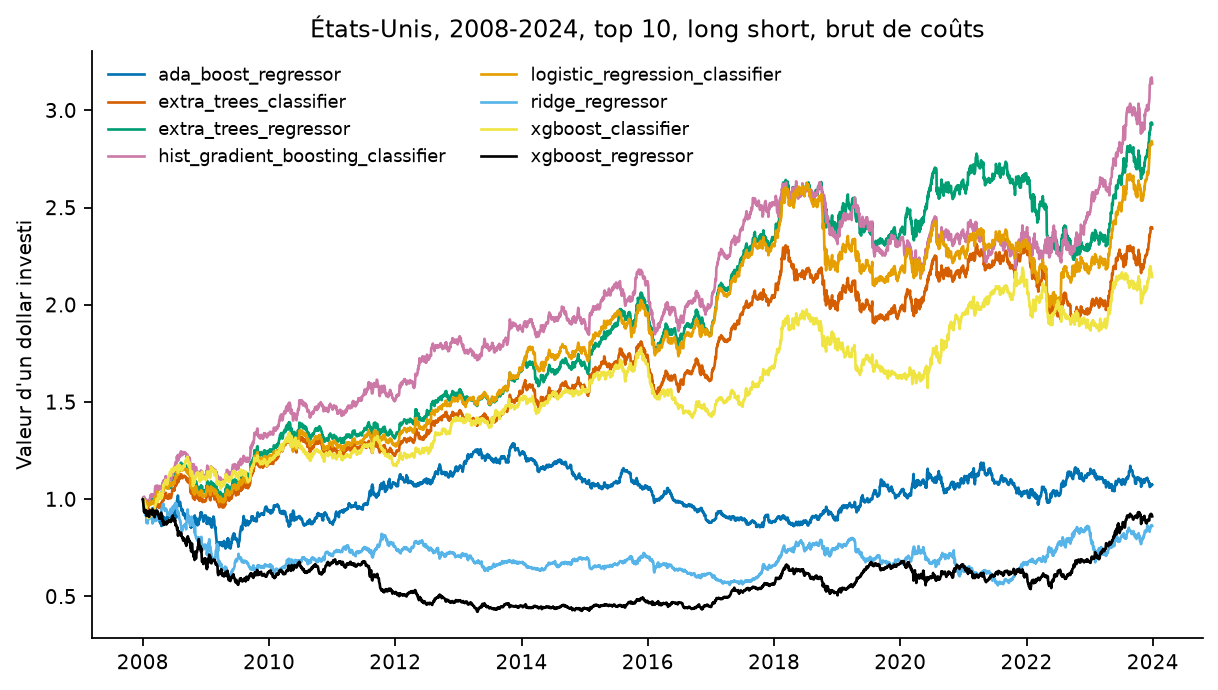
\includegraphics[width=.95\textwidth]{figures/usa_2008-2024_top10_corrected.png}
\caption{Croissance d'un dollar investi, portefeuilles long short top 10, États-Unis, 2008-01 à 2024-01, sans coûts.}
\end{figure}

\begin{figure}[h]
\centering
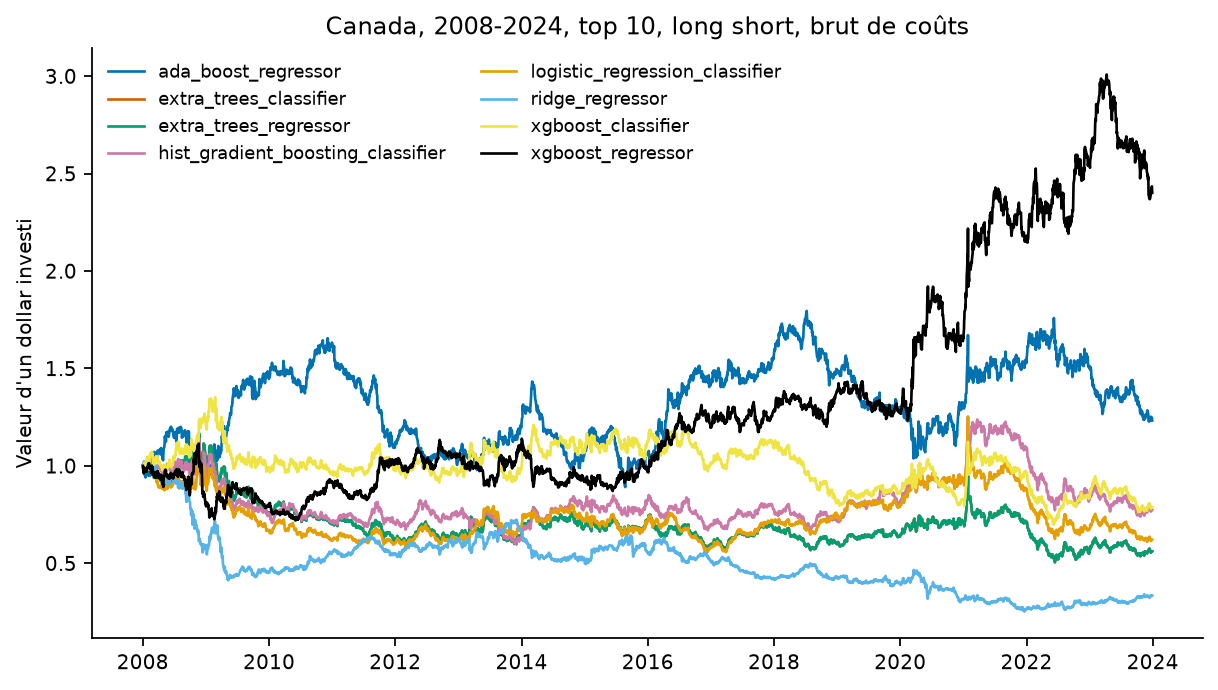
\includegraphics[width=.95\textwidth]{figures/canada_2008-2024_top10_corrected.png}
\caption{Croissance d'un dollar investi, portefeuilles long short top 10, Canada (50 titres), 2008-01 à 2024-01, sans coûts.}
\end{figure}

\clearpage
\begin{figure}[h]
\centering
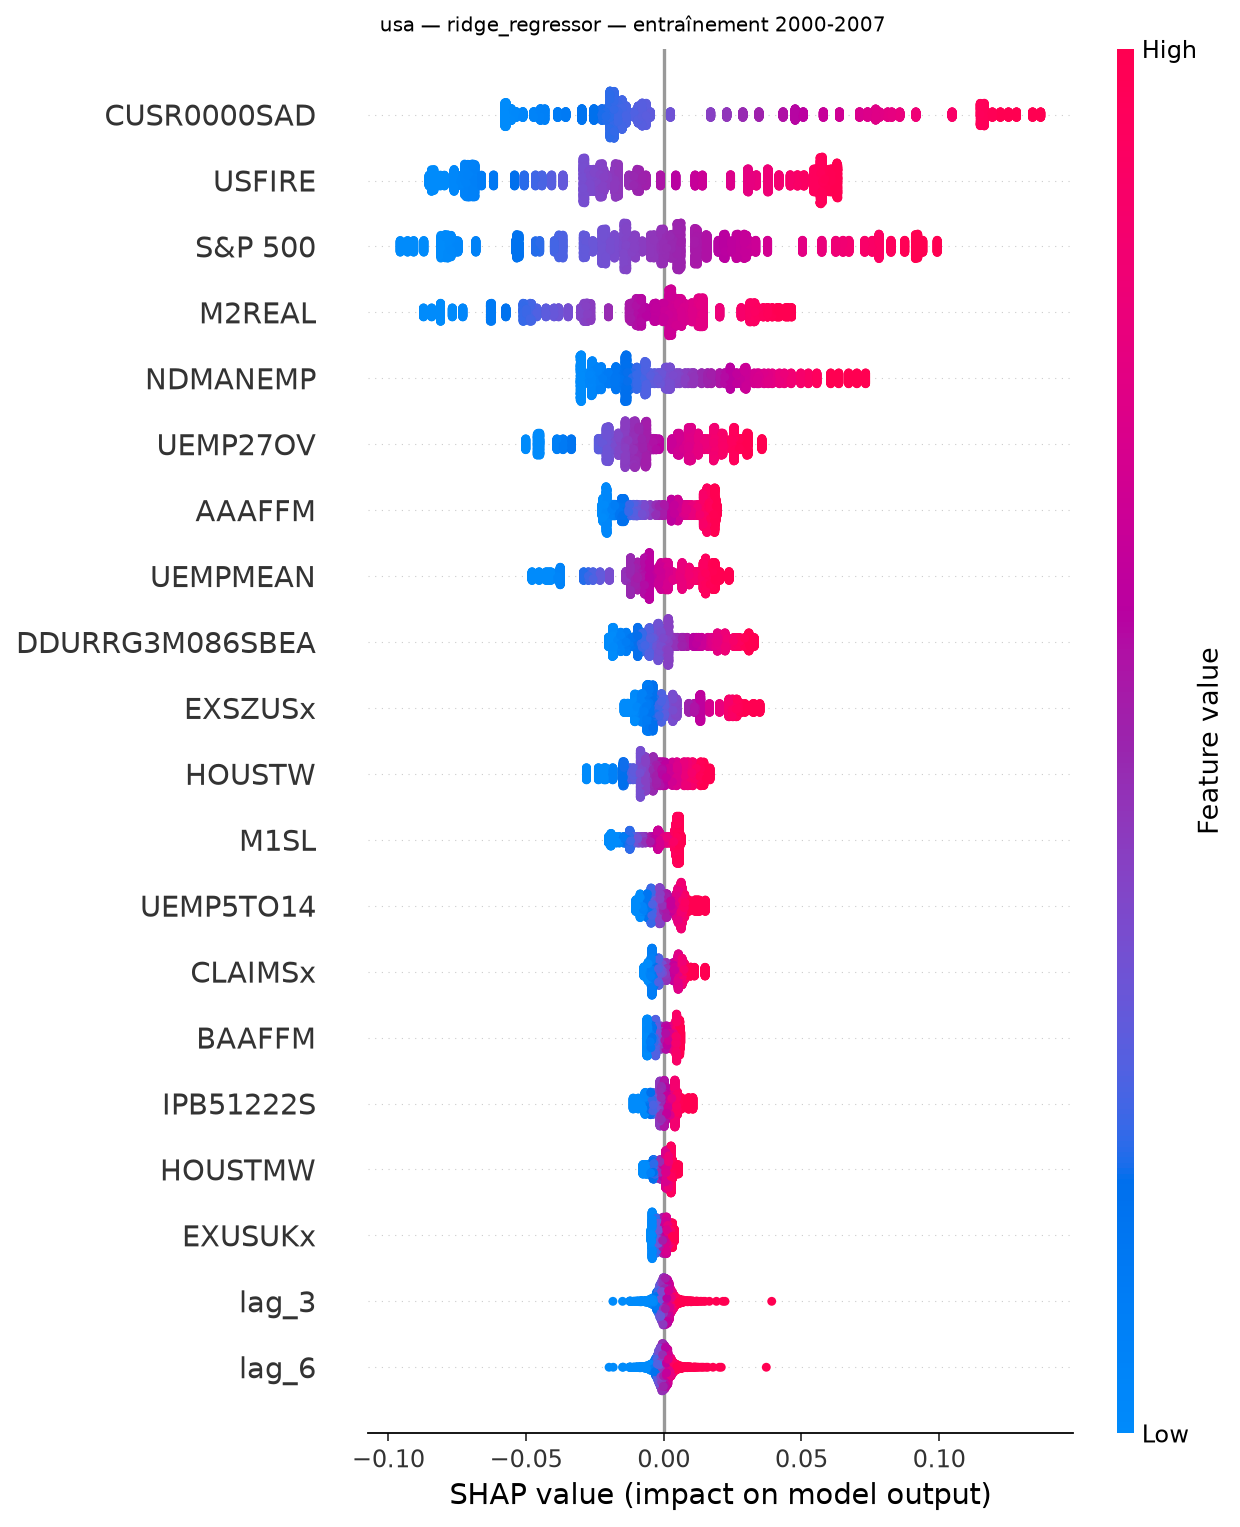
\includegraphics[width=.8\textwidth]{figures/shap_usa_summary_ridge_regressor.png}
\caption{Importance des variables par SHAP, Ridge, États-Unis, période d'entraînement 2000-2007. Chaque point est
une observation (un titre, un mois) ; la position horizontale donne la contribution à la prédiction, la couleur la
valeur de la variable. Contrairement aux figures de 2024, les contributions sont empilées entre les titres et non
moyennées, et le modèle expliqué porte les hyperparamètres retenus par la recherche bayésienne.}
\end{figure}

\begin{figure}[h]
\centering
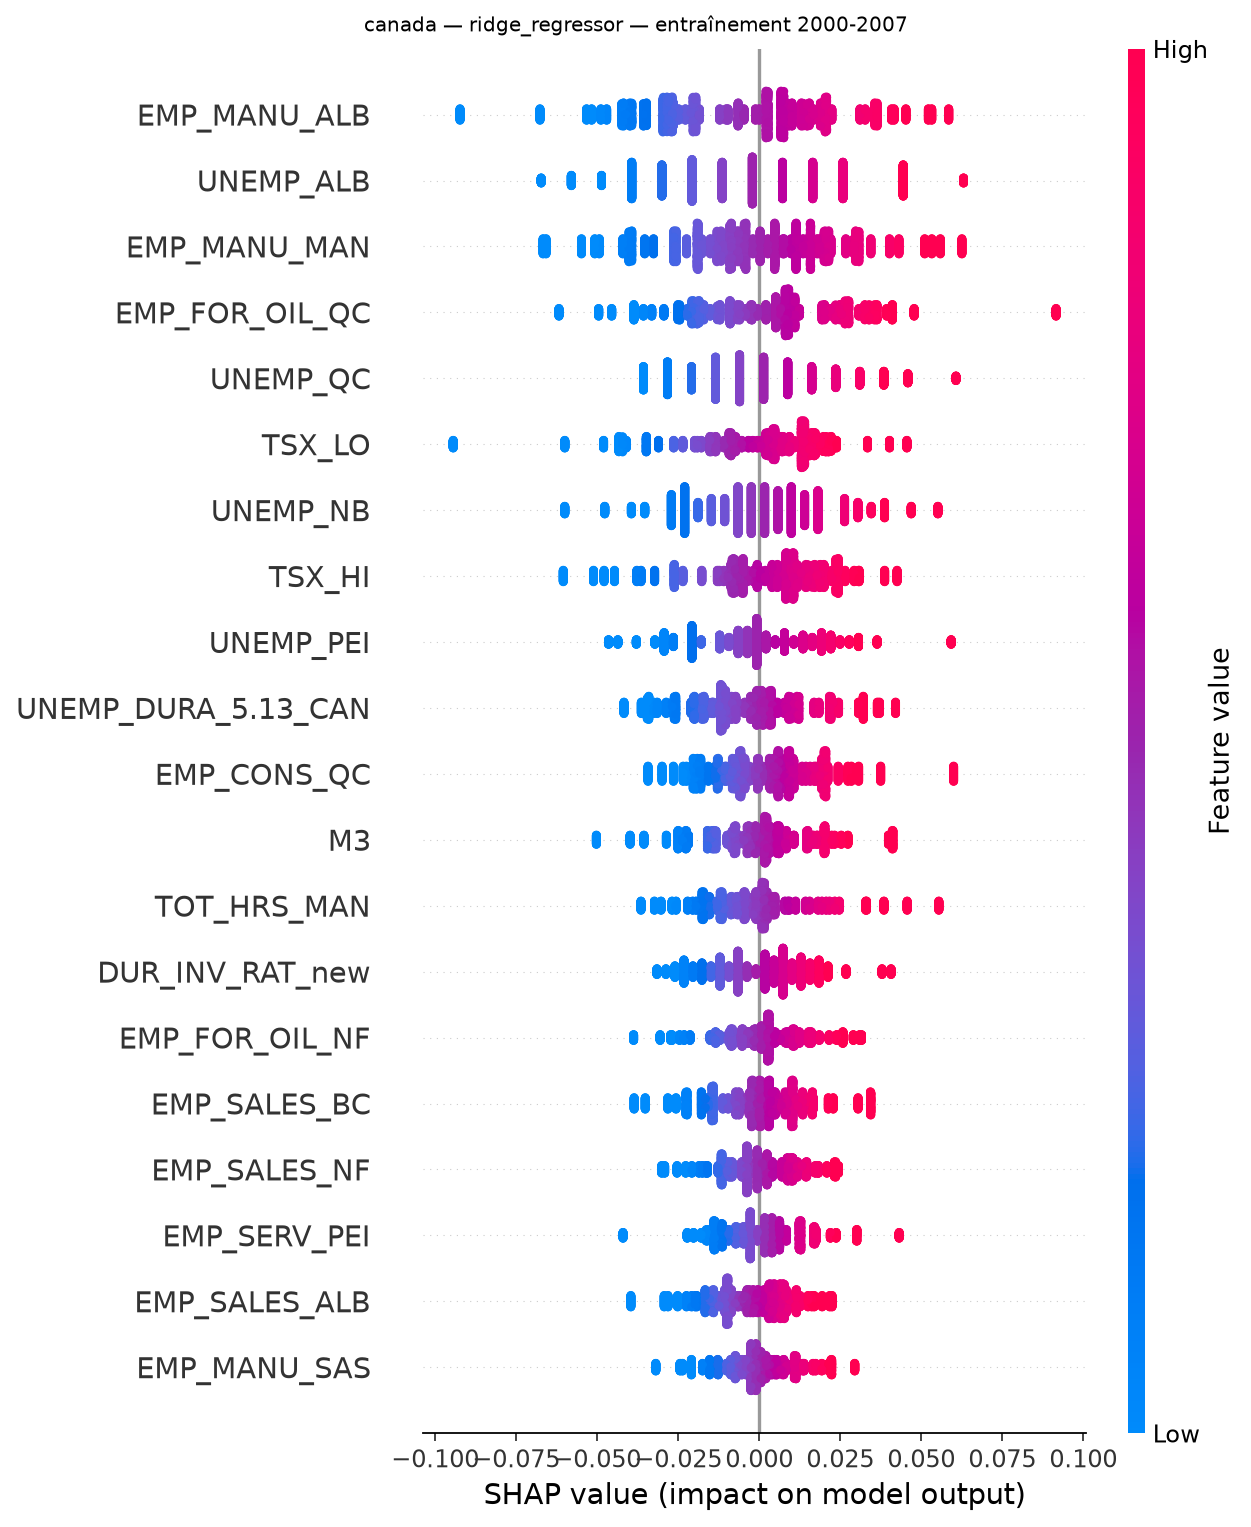
\includegraphics[width=.8\textwidth]{figures/shap_canada_summary_ridge_regressor.png}
\caption{Importance des variables par SHAP, Ridge, Canada (50 titres), période d'entraînement 2000-2007.}
\end{figure}

\end{document}
